
%----------------------------------------------------------------------------------------
%	PACKAGES AND OTHER DOCUMENT CONFIGURATIONS
%----------------------------------------------------------------------------------------

\documentclass[landscape,a0paper,fontscale=0.335]{baposter} % Adjust the font scale/size here

\usepackage{graphicx} % Required for including images
\graphicspath{{figures/}} % Directory in which figures are stored

\usepackage{amsmath} % For typesetting math
\usepackage{amssymb} % Adds new symbols to be used in math mode

\usepackage{booktabs} % Top and bottom rules for tables
\usepackage{enumitem} % Used to reduce itemize/enumerate spacing
\usepackage{palatino} % Use the Palatino font
\usepackage[font=small,labelfont=bf]{caption} % Required for specifying captions to tables and figures

\usepackage{multicol} % Required for multiple columns
\setlength{\columnsep}{1.5em} % Slightly increase the space between columns
\setlength{\columnseprule}{0mm} % No horizontal rule between columns

\usepackage{tikz} % Required for flow chart
\usetikzlibrary{shapes,arrows} % Tikz libraries required for the flow chart in the template

\newcommand{\compresslist}{ % Define a command to reduce spacing within itemize/enumerate environments, this is used right after \begin{itemize} or \begin{enumerate}
\setlength{\itemsep}{1pt}
\setlength{\parskip}{0pt}
\setlength{\parsep}{0pt}
}

\definecolor{red}{rgb}{1.00,0.14,0.14} % Defines the color used for content box headers

\begin{document}

\begin{poster}
{
headerborder=closed, % Adds a border around the header of content boxes
colspacing=1em, % Column spacing
bgColorOne=white, % Background color for the gradient on the left side of the poster
bgColorTwo=white, % Background color for the gradient on the right side of the poster
borderColor=red, % Border color
headerColorOne=black, % Background color for the header in the content boxes (left side)
headerColorTwo=red, % Background color for the header in the content boxes (right side)
headerFontColor=white, % Text color for the header text in the content boxes
boxColorOne=white, % Background color of the content boxes
textborder=roundedright, % Format of the border around content boxes, can be: none, bars, coils, triangles, rectangle, rounded, roundedsmall, roundedright or faded
eyecatcher=true, % Set to false for ignoring the left logo in the title and move the title left
headerheight=0.1\textheight, % Height of the header
headershape=roundedright, % Specify the rounded corner in the content box headers, can be: rectangle, small-rounded, roundedright, roundedleft or rounded
headerfont=\Large\bf\textsc, % Large, bold and sans serif font in the headers of content boxes
%textfont={\setlength{\parindent}{1.5em}}, % Uncomment for paragraph indentation
linewidth=2pt % Width of the border lines around content boxes
}
%----------------------------------------------------------------------------------------
%	TITLE SECTION 
%----------------------------------------------------------------------------------------
%
{\includegraphics[height=4em]{Austin_Peay_Governors_logo.png}} % First university/lab logo on the left
{\bf\textsc{Analysis of a simply supported beam}\vspace{0.5em}} % Poster title
{\textsc{ Joseph Spear - Austin Peay State University - Department of Physics, Engineering, and Astronomy}} % Author names and institution
{\includegraphics[height=4em]{Austin_Peay_Governors_logo.png}} % Second university/lab logo on the right

%----------------------------------------------------------------------------------------
%	Abstract
%----------------------------------------------------------------------------------------
%
\headerbox{Abstract}{name=abstract,column=0,span=2,row=0}{


The studying of the mechanics of various materials leads to the ability to theoretically find the maximum allowable load materials may withstand. In this computational study, a concrete beam of length $L=30m$ and height $h=6m$ is subject to an evenly distributed load $q$ which causes it to bend under the load. An increasing load creates a larger stress throughout the entire beam, until it fractures due to a small crack at $x = \frac{L}{2}$. This fracture occurs when the load distribution exceeds $F = 63833 \frac{N}{m}$, causing the concrete to fail in tension.


\vspace{0.3em} % When there are two boxes, some whitespace may need to be added if the one on the right has more content
}

%----------------------------------------------------------------------------------------
%	OBJECTIVES
%----------------------------------------------------------------------------------------

\headerbox{Introduction}{name=objectives,column=0,span=2, below=abstract}{

The study of the \textit{Mechanics of Materials} allows for various properties of structural components, such as beams, to be analyzed. The goal of \textit{Mechanics of Materials} is to find mathematical relationships to describe the behavior of the structural components. In this computational experiment, the following properties are found:

\begin{multicols}{2}
\begin{enumerate}\compresslist
\item Stress associated with the beams geometry
\item The deflection curve of the beam
\item The associated Shear / Moment diagram
\item Maximum allowable Stress
\item Load at which fracture will occur
\end{enumerate}

\columnbreak

\begin{center}
\includegraphics[width=3.0in, height=1.0in]{SimpleBeam.png}
\scriptsize{
\\ Figure 1: Simply supported beam with even load distribution. \\
Image created by Joseph Spear on December 10, 2019
}
\end{center}


\end{multicols}


\vspace{0.3em} % When there are two boxes, some whitespace may need to be added if the one on the right has more content
}


%----------------------------------------------------------------------------------------
%	METHODOLOGY
%----------------------------------------------------------------------------------------

\headerbox{Methodology}{name=method,column=0,span=2,below=objectives}{ % This block's bottom aligns with the bottom of the conclusion block

In order to visualize the stresses acting on a beam under this type of load, the principles of static structures must be used by observing the beams free body diagram, and applying Newton's Second Law in Static Equilibrium:

\begin{equation}
\Sigma F = 0
\label{eq: SumForces}
\end{equation}\

Once this is completed, the beam may be cut into a "section" and the internal shear force and internal moment may be found using the Left Hand - Free Body Diagram. Equations (2) and (3) are found in this manner, and Equation (4) is the relationship between the deflection $\left(\nu\right)$ and the internal Moment (Goodno, 449 \& 1107).

\begin{multicols}{3}
\begin{equation}
V(x) = \frac{qL}{2} - qx
\label{eq: Shears}
\end{equation}\


\begin{equation}
M(x) = - \frac{q}{2}x^2 + \frac{qL}{2}x 
\label{eq: Moments}
\end{equation}\


\begin{equation}
\frac{d^2\nu}{dx^2} = \frac{M(x)}{EI}
\label{eq: Deflection}
\end{equation}\

\end{multicols}

For analysis of beam failure, a few assumptions must be made. The first is that a concrete mix with a fracture toughness of $K_{Ic} = 1.0 MPa\sqrt{m}$ is used. It is also assumed that the associated geometric parameter is assumed to be $Y=1$. Lastly, the assumed initial crack radius is $a = 0.5$. With these parameters in place, the following relation may be used to calculate the critical fracture stress (Callister,334):

\begin{equation}
\sigma_c = \frac{K_{Ic}}{Y\sqrt{\pi a}}
\label{eq: CrackStress}
\end{equation}\


}

%----------------------------------------------------------------------------------------
%	Acknowledgements and Future Wokrs
%----------------------------------------------------------------------------------------

\headerbox{Acknowledgments \& Further Works}{name=acknowledge,column=0, span=2,row=0, above=bottom, below=method}{

Special thanks to Dr. Oelgoetz and Dr. Lonnghurst for their guidance in these topics!\\

In further pursuit of this topic, an in depth study of crack propagation over time due to fatigue cycles would be desired. This may be accomplished using a time-step approximation technique such as Euler's Method and would yield interesting and useful results. The same process used in this study may also be performed for a wide range of materials and loads to produce more intricate and realistic cases. 

}


%----------------------------------------------------------------------------------------
%	CONCLUSION
%----------------------------------------------------------------------------------------

\headerbox{Results \& Conclusion}{name=conclusion,column=2,span=2,row=0, bottomaligned=method}{ %,above=references
\setlength{\columnsep}{1pt}
\begin{multicols}{2}

\begin{itemize}
\item Figure 2 represents the side-view of the beam, where the distributed load (q) is applied to the top face of the beam. In this situation, the symmetric load causes the concrete to bend down towards the middle which in turn causes a stress in compression on the top face (indicated with dark blue), and a stress in tension on the bottom face (yellow). The center of the beam remains a constant color, indicating what is known as the neutral axis, where the stress is zero.
\end{itemize}

\columnbreak

\begin{center}
\includegraphics[width=\linewidth, height=1.6in]{StressDistribution1.eps}
\scriptsize{
Figure 2: Stress Distribution throughout the Beam
}
\end{center}

\end{multicols}


\begin{multicols}{2}
\begin{center}
\includegraphics[width=\linewidth, height=1.6in]{Shear_Moment.eps}
\scriptsize{
Figure 3: Shear-Moment Diagram of the Beam
}
\end{center}
 
\columnbreak 
 
\begin{itemize}
\item The internal Shear and bending Moment of a material is extremely important in design and in determining other properties. Equation (4) wouldn't be solvable without Equation (3)! Therefore, a useful tool to help with the analysis of materials is the \textit{Shear-Moment Diagram}. This diagram models the internal shear and bending moments felt throughout the beam, and helps determine maximum and minimum points of stress.
\end{itemize}

\end{multicols}

\begin{multicols}{2}

\begin{itemize}
\item Due to the solution of Equation (4), the deflection curves for various loads may be modeled. These deflections show the neutral axis after the load is applied, and is contrasted by the load-free neutral axis in black. The deflection curve is an important property which can be used for various applications, such as understanding the ductility of a beam or designing a beam which will not fracture. Deflection is also an observable quantity making it useful in an applied setting.
\end{itemize}

\columnbreak

\begin{center}
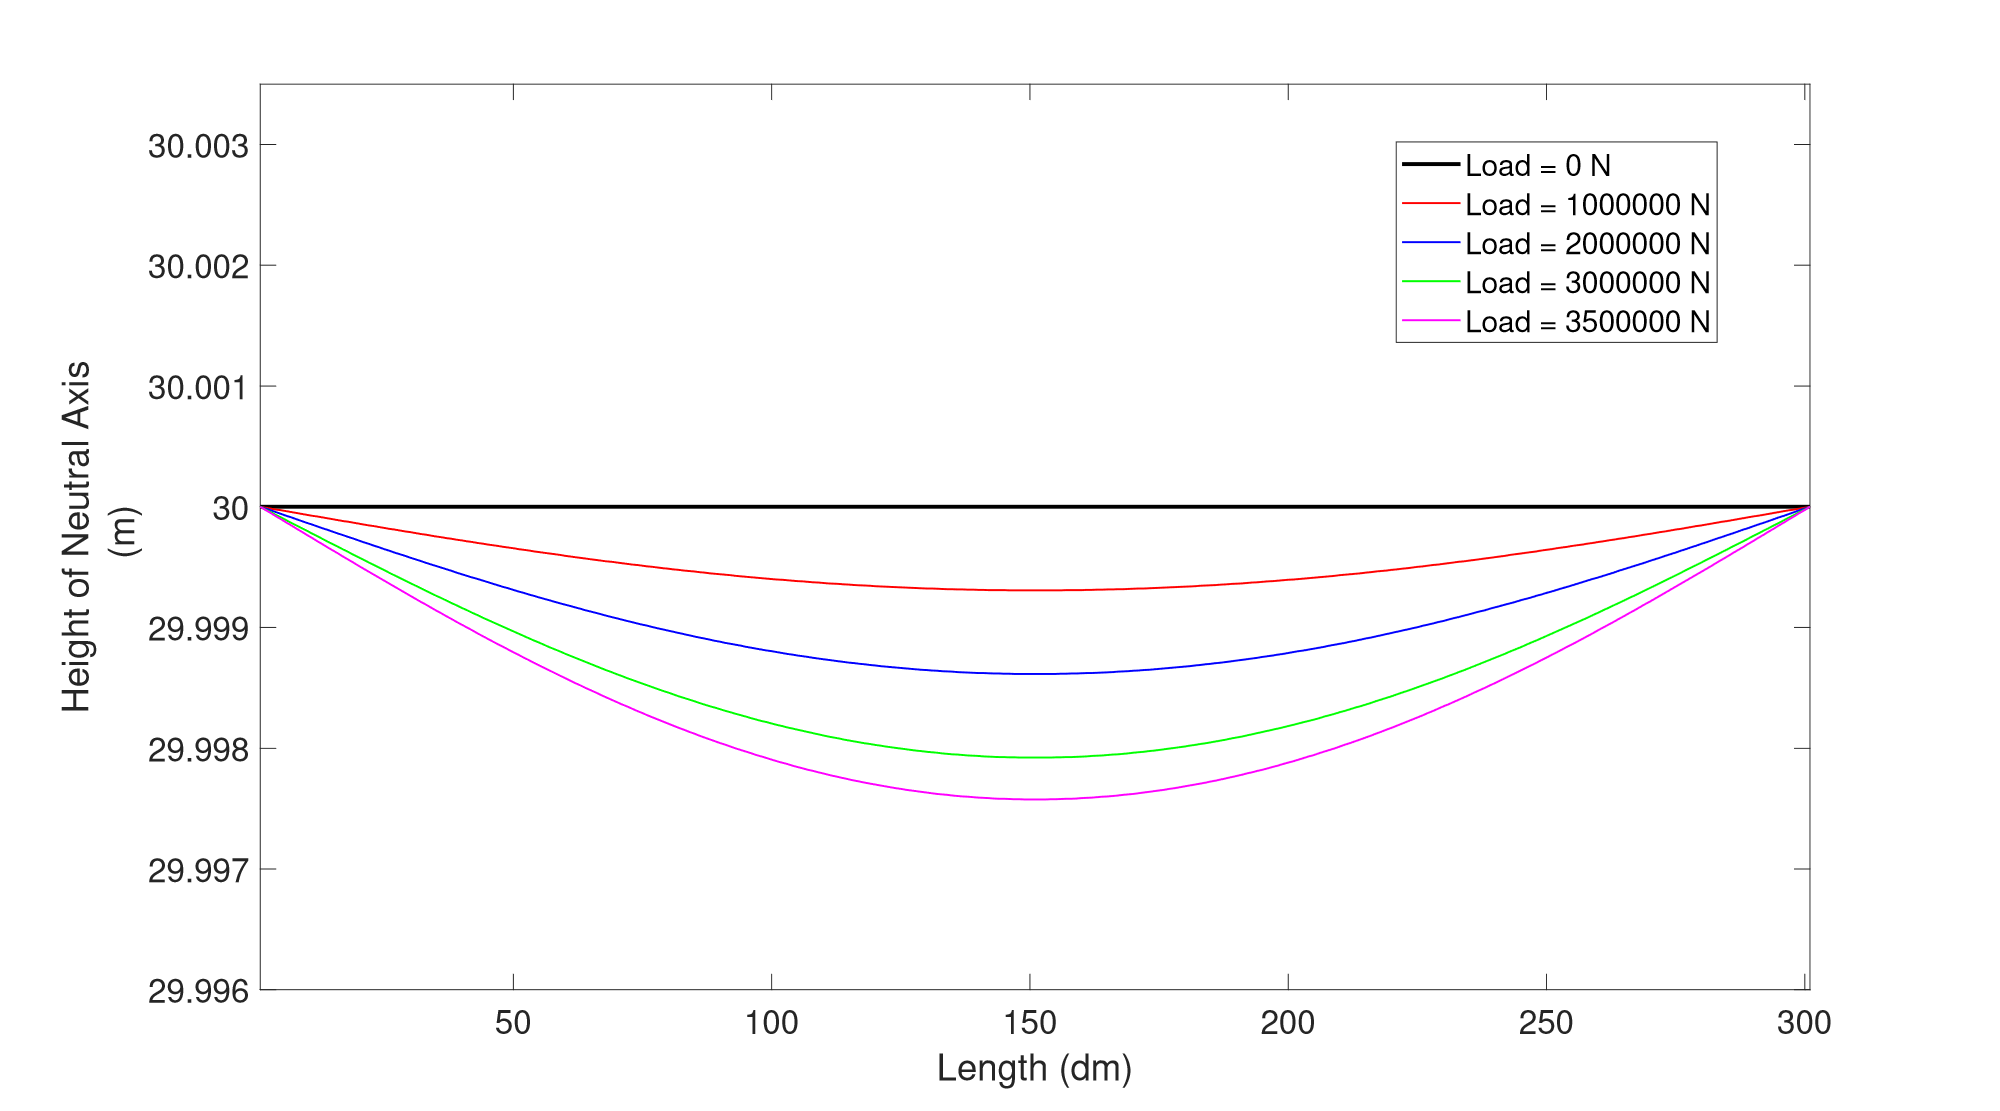
\includegraphics[width=\linewidth, height=1.6in]{Deflection.eps}
\scriptsize{
Figure 4: Deflection Relative to the Neutral Axis
}
\end{center}

\end{multicols}



Based on the previous information, specifically Equation (5), it is determined that the theoretical concrete mix would fracture in tension on the bottom face given the following conditions:\\

\center $\sigma_{allowable} = 1784124.0913288831 \hspace{0.055in} Pa$  ;\hspace{0.45in} $q_{max} = 63833 \hspace{0.055in} \frac{N}{m}$  ;\hspace{0.45in}  $\delta = 1.326259670491936 \hspace{0.055in} mm$;   \hspace{0.45in}    $a_o = 0.5\hspace{0.055in} m$

\vspace{0.2in}
\begin{flushleft} 
These quantities would allow engineers to design safe structures using cheap computations instead of costly experiments. This process may also be performed with any type of load or material desired, as long as the boundary conditions are known.
\end{flushleft}

}

%----------------------------------------------------------------------------------------
%	REFERENCES
%----------------------------------------------------------------------------------------

\headerbox{References}{name=references,column=2, span=2,row=0,above=bottom, below=conclusion}{
% Include references for bapsoter, AP Logo, Mechanics of Materials Book, Material Science Book

\begin{enumerate}

\item Amberg, Brian \textit{The baposter latex poster style}, 2011, http://www.brian-amberg.de/uni/poster/ Accessed 10 Dec. 2019.

\item Goodno, Barry J., James Gere, \textit{Mechanics of Materials: Ninth Edition} Boston, MA, Cengage Learning, 2018.

\item Callister, William D., David Rethwisch, \textit{Fundamentals of Materials Science and Engineering} Danvers, MA, John Wiley \& Sons, Inc., 2015.

\end{enumerate}

}

\end{poster}

\end{document}
